\documentclass[a4paper]{IEEEtran}

\usepackage{xcolor}
\usepackage{hyperref}
\usepackage[utf8]{inputenc}
\usepackage[pdftex]{graphicx} 
\usepackage{pdfpages}
\usepackage{multirow, pgfplotstable,booktabs,colortbl,lmodern}
\usepackage{mathtools}
\usepackage{listings}
\usepackage{color}

\definecolor{dkgreen}{rgb}{0,0.6,0}
\definecolor{gray}{rgb}{0.5,0.5,0.5}
\definecolor{mauve}{rgb}{0.58,0,0.82}

\lstset{frame=tb,
    language=VHDL,
    aboveskip=3mm,
    belowskip=3mm,
    showstringspaces=false,
    columns=flexible,
    basicstyle={\small\ttfamily},
    numbers=none,
    numberstyle=\tiny\color{gray},
    keywordstyle=\color{blue},
    commentstyle=\color{dkgreen},
    stringstyle=\color{mauve},
    breaklines=true,
    breakatwhitespace=true
    tabsize=3
}

\newcommand\TODO[1]{\textcolor{red}{TODO:#1}}
\newcommand\todo[1]{\TODO{#1}}
\newcommand\cn{\textcolor{red}{[citation needed]}}

\begin{document}

\begin{titlepage}

    \newcommand{\HRule}{\rule{\linewidth}{0.5mm}} % Defines a new command for the horizontal lines, change thickness here

    \center % Center everything on the page

    \vspace*{2cm}

    %----------------------------------------------------------------------------------------
    %   HEADING SECTIONS
    %----------------------------------------------------------------------------------------

    \textsc{\LARGE Norwegian University of Science and Technology}\\[1.5cm] % Name of your university/college
    \vspace*{1cm}
    \textsc{\Large Term assignment}\\[0.5cm] % Major heading such as course name
    \textsc{\large TFE4140 Modeling and Analysis of Digital Systems}\\[0.5cm] % Minor heading such as course title
    \vspace*{1.4cm}

    %----------------------------------------------------------------------------------------
    %   TITLE SECTION
    %----------------------------------------------------------------------------------------

    \HRule \\[0.4cm]
    { \huge \bfseries Liaison}\\[0.4cm] % Title of your document
    \textsc{\large A fault tolerant communication system}\\[0.5cm] % Minor heading such as course title
    \HRule \\[1.5cm]

    %----------------------------------------------------------------------------------------
    %   AUTHOR SECTION
    %----------------------------------------------------------------------------------------
    \vspace*{1cm}

    \begin{minipage}{0.4\textwidth}
        \begin{flushleft} \large
            \emph{Author:}\\
            Rune \textsc{Holmgren} \newline% Your name
            Torbjørn \textsc{Langland} % Your name
        \end{flushleft}
    \end{minipage}
    ~
    \begin{minipage}{0.4\textwidth}
        \begin{flushright} \large
            \emph{} \\
            \textsc{} % Supervisor's Name
        \end{flushright}
    \end{minipage}\\[4cm]

    % If you don't want a supervisor, uncomment the two lines below and remove the section above
    %\Large \emph{Author:}\\
    %John \textsc{Smith}\\[3cm] % Your name

    %----------------------------------------------------------------------------------------
    %   DATE SECTION
    %----------------------------------------------------------------------------------------

    \vspace*{2cm}
    {\large \today}\\[3cm] % Date, change the \today to a set date if you want to be precise

    %----------------------------------------------------------------------------------------
    %   LOGO SECTION
    %----------------------------------------------------------------------------------------

    %\includegraphics{Logo}\\[1cm] % Include a department/university logo - this will require the graphicx package

    %----------------------------------------------------------------------------------------

    \vfill % Fill the rest of the page with whitespace

\end{titlepage}
\clearpage

\begin{titlepage}
    \vspace*{2cm}
    \begin{abstract}
        \todo{ Compulsory (means that it is specified in the Term Project in description of report set up, and at this very location). Create a fitting abstract here. Also create a FRONT PAGE. Yes, you didn't read wrong. I wrote in capital letters. If we miss this now, we must indeed be quite stupid...}

    \end{abstract}
\end{titlepage}

\clearpage

\begin{titlepage}
    \tableofcontents
\end{titlepage}

\clearpage

\section{Introduction}
When technology is brought into extreme enviroments, it need to be designed to withstand that enviroment.
The new NTNU student satelite is a good example of such a technological product.
The heavy radiation in space will affect the onboard computer system, and can at any time break it.
The likelyhood of such a catastrophic failiure can however be reduced significantly by indrodusing redundancy to the system.
This redundance is to be managed by the liaison module, as described in this paper.
The module allow the system to run 4 identical microcontrollers, and compare the outputs to each other.
Anytime a microcontroller fails, the Liaison system will notice the fault by comparing the microcontrollers outputs.
The failed microcontroller will then be ignored for the rest of the systems lifetime, while the other microcontrollers will be able to continue working.
By allowing the system to work even at just two non-faulty microcontrollers, the system have an improved expected life time.
In addition to faulty microcontrollers, the radiation of space introduce a risk of bit errors in transmissions back to earth.
The system will have to add error correcting and detecting bits to each transmission back to earth, that can then be used to verify and potentially correct the data.
This is achived through use of Hamming code.
\break
This report presents the solution for the Liasion system designed by group 1.
Chapter 2 presents the problem and all required functionality in details.
Chapter 3 presents the technical solutions to the problem, split into different sub-problems according to the Term Assignment paper\cite{assignment-text}.
Chapter 4 presents the testing and verification that is done of the product.
Chapter 5 presents the results from synthesizing the product.
Chapters 6 and 7 adds additional information and concludes the report.

\section{Problem}

\subsection{The Liasion Fault Tolerant System}
NTNU is working with a Student Satellite, which is to orbit Earth and measure atmospheric data and deliver this to a ground stattion.
The goal of this Assignment is to design a fault tolerant system called Liasion, which exploits redundancy.
The system will contain four independent microcontrollers, that perform the same calculations.
Every computation will procude 8-bit words.
There is always the chance due to cosmic radiation that one more microcontrollers may produce incorrect data.
If this is the case, the majority will decide the correct data, in a \textit{voting} process.
The voted data is to be accompanied by a 3-bit status signal which contains the number of failed microcontrollers.
If too many microcontrollers have failed, this status signal will indicate it so that recieved data cannot be trusted.
Additionally, data may be corrupted before reaching Earth.
This problem is to be solved by implementing a module with Error Correcting Circuit (ECC) that uses Hamming Code.
The chosen solution must be able to correct single-bit errors and detect double-bit errors\protect\cite{assignment-text}.

\subsection{The Liasion Module functionality in details}

\begin{figure}[h!]
    \centering
    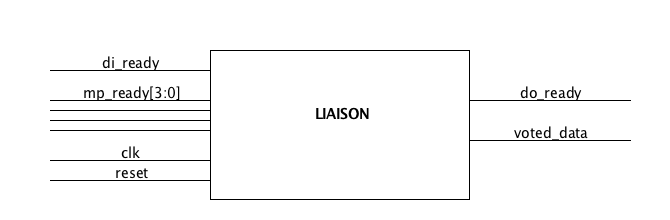
\includegraphics[width=0.5\textwidth]{Figures/ProjectDescription/LiaisonBlackBox}
    \caption{The Liaison module with inputs and outputs (reprinted from \protect\cite{assignment-text}).}
    \label{fig:LiaisonBlackBox}
\end{figure}

Figure \ref{fig:LiaisonBlackBox} shows the Liaison module with the inputs and outputs that are specified for the procject:
\begin{itemize}
    \item \textbf{di\_ready}: A pulse that warns the module that data starts arriving from the microcontrollers. Active high.
    \item \textbf{mp\_data}: input from the microcontrollers. The bus is 4 bits wide, one bit for each microcontroller. The bits arrive serially, with MSB arriving first.
    \item \textbf{reset}: Synchronous reset of the system. Active high.
    \item \textbf{clk}: Clock. All flip-flops are clocked on the positive edge of the clock.
    \item \textbf{do\_ready}: A output pulse that indicates that data starts arriving from the Liasion to the receiver, through the output \textit{voted\_data}.
    \item  \textbf{voted\_data}: The voted result (8 bits) are sent out, clocked and serially, followed by status bits (3 bits) and error correction code (m bits).
        MSB first.
        This can be seen in figure \ref{fig:LiaisonOutput}, where it will take 11+m cycles for a full set of data package to be sent out.
\end{itemize}

\begin{figure}[h!]
    \centering
    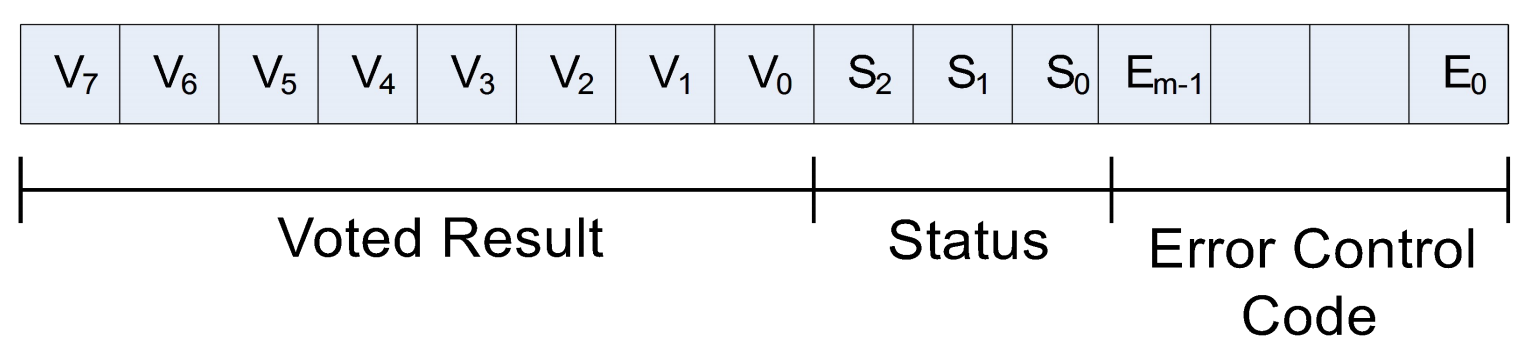
\includegraphics[width=0.5\textwidth]{Figures/ProjectDescription/LiaisonOutput}
    \caption{The total output of data (reprinted from \protect\cite{assignment-text}).}
    \label{fig:LiaisonOutput}
\end{figure}

\begin{figure}[h!]
    \centering
    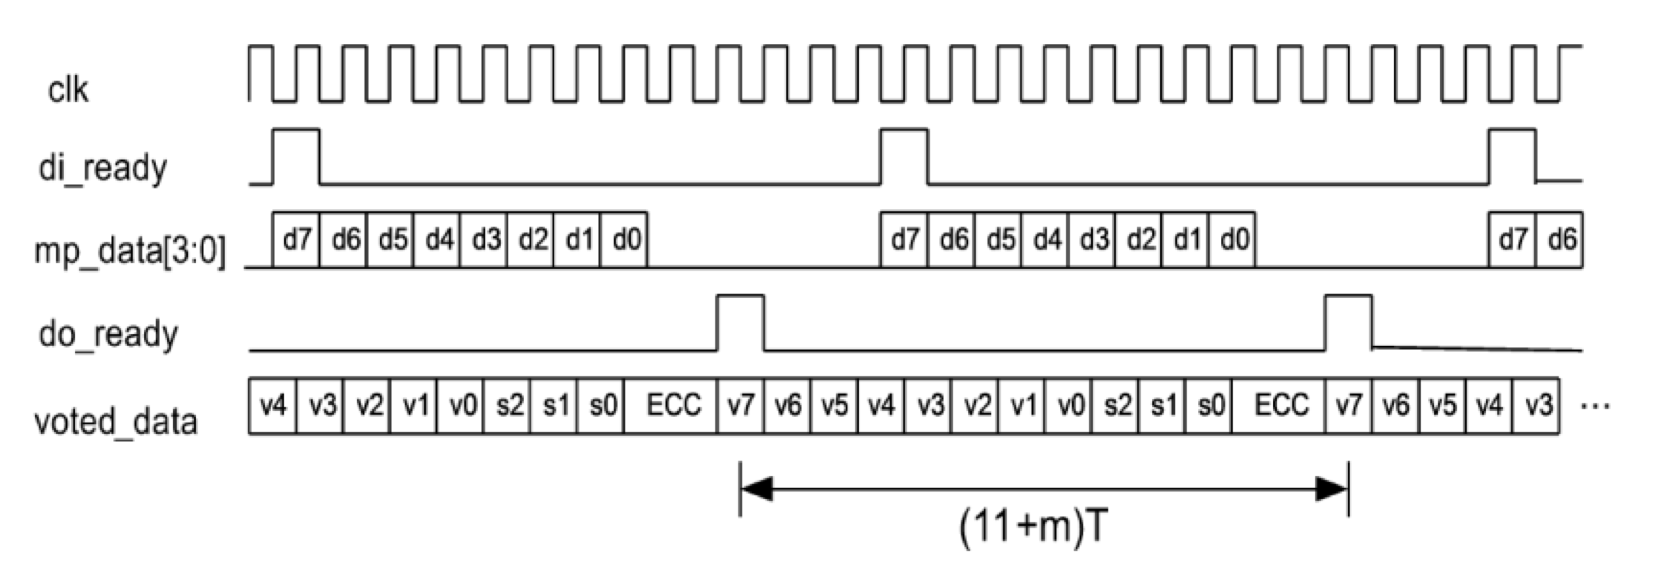
\includegraphics[width=0.5\textwidth]{Figures/ProjectDescription/LiaisonInputOutput}
    \caption{The relationship between the inputs and the outputs of the module (reprinted from \protect\cite{assignment-text}).}
    \label{fig:LiaisonInputOutput}
\end{figure}

Figure \ref{fig:LiaisonInputOutput} shows the system operating with maximum throughput, and it can be seen that there are some delays in the inputs in order to allow the maximum throughput.
Since the Liasion has to send more than just the voted data, it cannot store input data constantly.

\begin{figure}[h!]
    \centering
    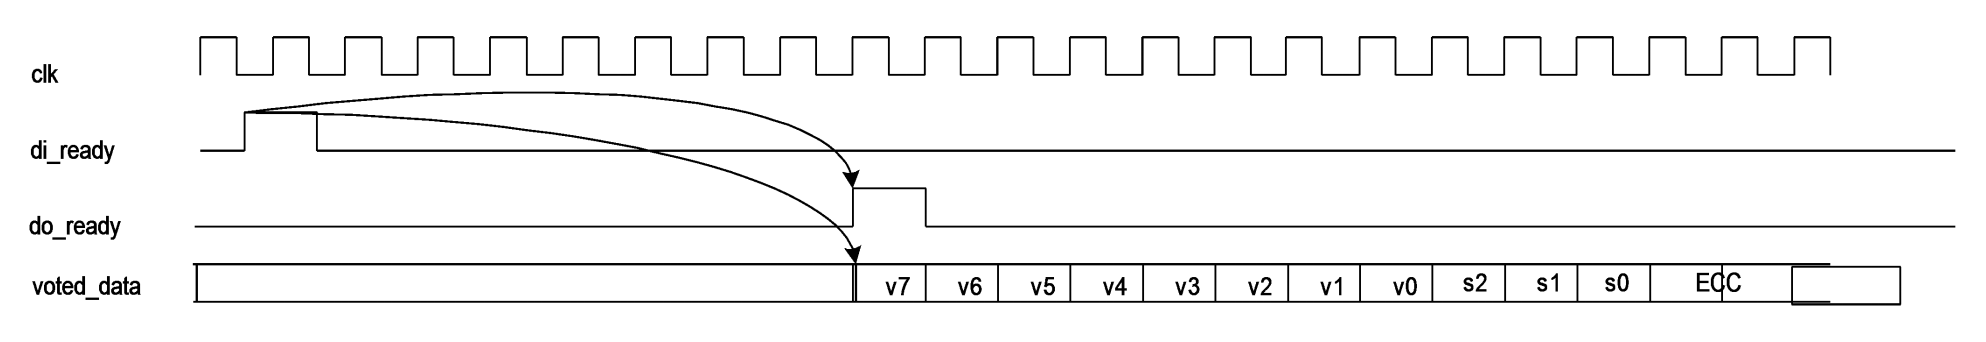
\includegraphics[width=0.5\textwidth]{Figures/ProjectDescription/LiaisonDiReadyDoReady}
    \caption{A pulse of di\_ready causes a do\_ready pulse after n cycles (reprinted from \protect\cite{assignment-text}).}
    \label{fig:LiaisonDiReadyDoReady}
\end{figure}

Figure \ref{fig:LiaisonDiReadyDoReady} shows that there are some delay between \textit{di\_ready} and \textit{do\_ready} that is specified by m cycles.
The latter must be caused by the first, and output data must be sent from the moment \textit{do\_ready} pulses.

\begin{figure}[h!]
    \centering
    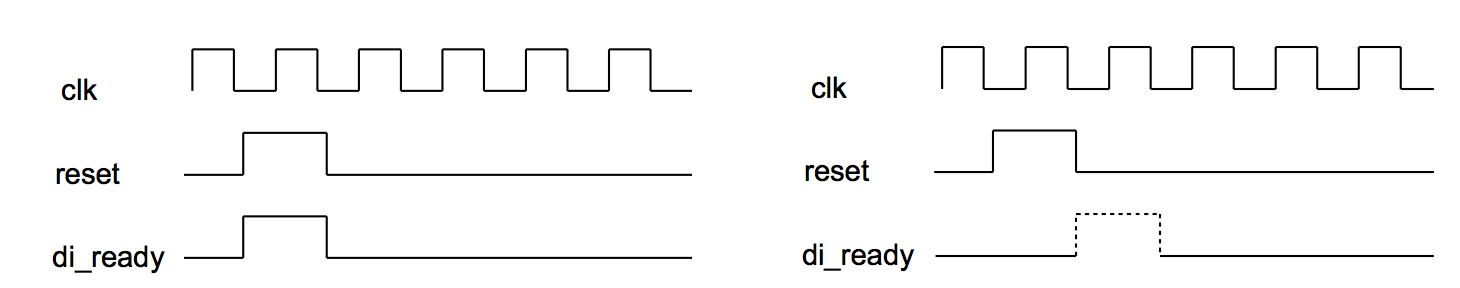
\includegraphics[width=0.5\textwidth]{Figures/ProjectDescription/LiaisonResetDiReady}
    \caption{Reset has precedence over di\_ready (reprinted from \protect\cite{assignment-text}).}
    \label{fig:LiaisonResetDiReady}
\end{figure}

Figure \ref{fig:LiaisonResetDiReady} shows that the \textit{reset} signal must have precedence over the \textit{di\_ready} signal. Liaison must be ready to recieve data immediatly when \textit{reset} is no longer active.

\begin{figure}[h!]
    \centering
    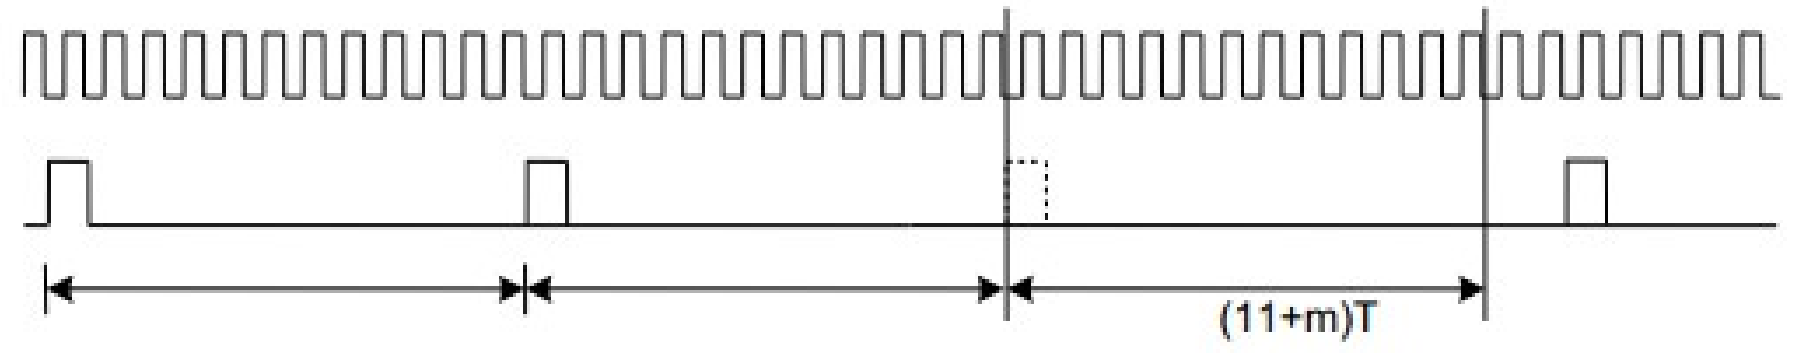
\includegraphics[width=0.5\textwidth]{Figures/ProjectDescription/LiaisonMaxThroughput}
    \caption{The maximum throughput is 11+m, each di\_ready signals may not arrive sooner than that (reprinted from \protect\cite{assignment-text}).}
    \label{fig:LiaisonMaxThroughput}
\end{figure}

Figure \ref{fig:LiaisonMaxThroughput} shows the intervals between the pulses of \textit{di\_ready}. The signal may arrive at any time, but there must be at least 11+m cycles between each interval.

\subsection{Project Framework}
The system is to be encoded in VHDL, tested and verified in simulation, and synthesized. A goal is to achieve as few Look Up Tables (LUTs) as possible. \todo{ Perhaps briefly explain what a LUT is?}
Active HDL 8.2 is used for programming in VHDL, as well as creating test benches and running simulations for verification.
Synplify Pro C-2009.06 is used for synthesizing, creating resulting LUTs and estimated frequency, and creating RTL view schematics and Technology view schematics. 
\\
\indent The Term Assignment was handed out at January 31st, 2014.
These are the milestones\protect\cite{assignment-text}:
\begin{itemize}
    \item \textbf{February 18th, 2014}: Assignment 3 of the Course, where the individual One-Bit Voters are designed. They serve as basis of the 8-bit voters
    \item \textbf{February 28th, 2014}: Delivery of technical notes, that will contain preliminary solutions to sub-problems 1, 2 and 3.
    \item \textbf{March 3rd, 2014}: Delivery of Peer Evaluation, containing evaluation of the technical note and project of another group.
    \item \textbf{March 31st}, 2014: Presentation of the project for groups 1-9 (minus 7).
    \item \textbf{April 3rd, 2014}: Presentation of the project for groups 7, 10-19.
    \item \textbf{April 4th, 2014}: Final report delivery.
\end{itemize}


\section{ Solution to the problem.}
This chapter will explain how the group has implemented the solution for the Term Assignment.
The Term Assignment was split into 5 sub-problems, therefore this report will detail the solution to each sub-problem accordingly.
This chapter explains the concept and functionality behind the design.

\subsection{Sub-Problem 1: State analysis}

The system begins with four working microcontrollers.
As time passes, one by one will fail.
First one microcontroller will fail, and it will be tagged as faulty.
It's input will be disregarded.
The next microcontroller breaks down after more time, and only two will remain.
When a third breaks down, the system will go into shutdown because there are no ways to know which one is correct.
This is implemented as a system state machine, and is illustrated in figure \ref{fig:StateMachine}.
\begin{figure}[h!]
    \centering
    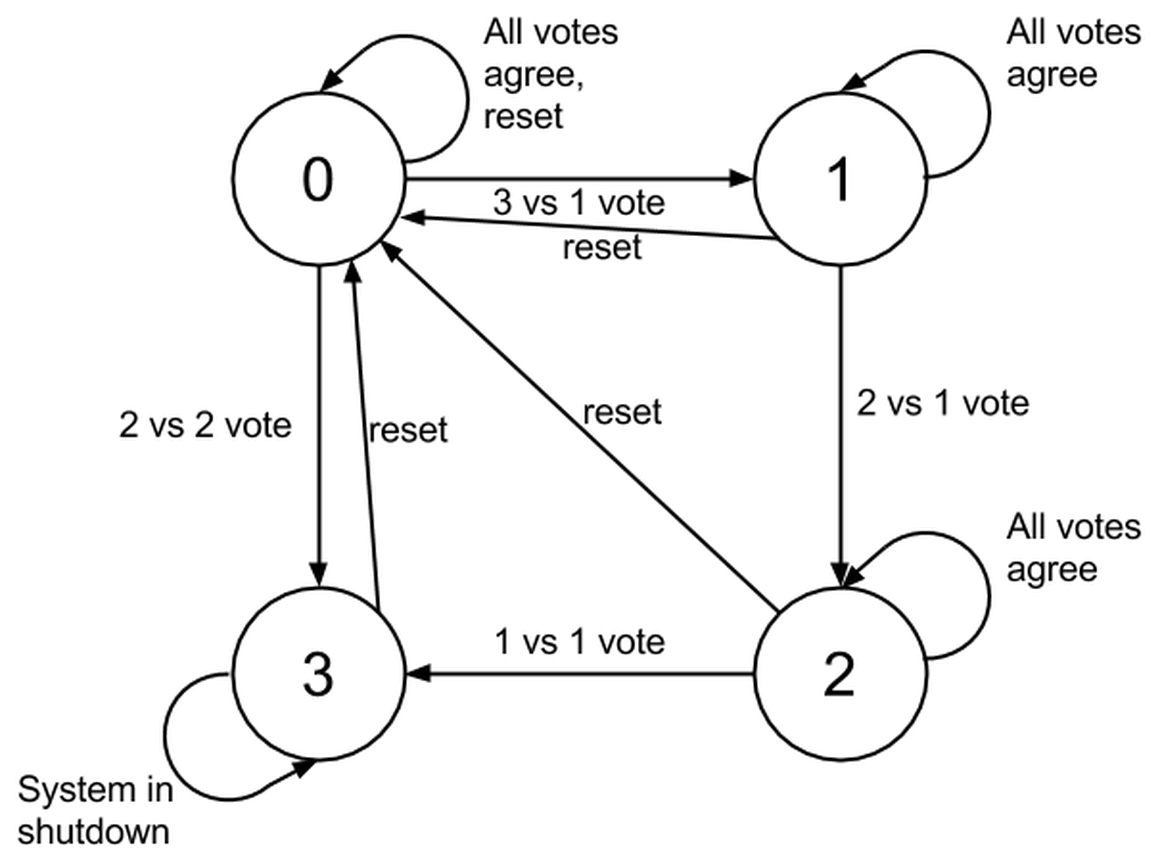
\includegraphics[width=0.5\textwidth]{Figures/Solution/StateMachine}
    \caption{System state machine.}
    \label{fig:StateMachine}
\end{figure}

As long as all microcontrollers agree, no one will be tagged for error and the system will remain in the same state.
For this system, the group has chosen to implement immediate error tagging as soon as an microcontroller disagree with the rest.
Another option could be to not implement error tagging until a series of errors pass and the pattern of errors is recognized.
But a microcontroller should never under any circumstanced disagree with the others as long as it is working, therefore the solution with immediatly error tagging is chosen.
This is also less complex to implement, saving the system for LUTs.
As one by one microcontroller fails, they are tagged and the status changes (expected from 0 to 1, 1 to 2 and 2 to 3).
There is also a special case, as can be seen in Figure \ref{fig:StateMachine}:
If two out of the four microcontrollers fail at the same time, the system will go to immediate shutdown, since it can no longer be known which two are working.
The probability for this to happen is very low, but let's say that something unprecedented happens, that damages the satellite (like if it is hit by a small meteorite).
If the damage affects two of the four microcontrollers, so that they disagree, then immediate shutdown would be needed.
The state diagram also shows that when reset occurs, the system returns to the initial state.
A 4-bit register, one bit for each microcontroller, is used to keep record of which microcontrollers work, and which don't.
The 3-bit status bits that the Liasion System sends out will contain data of how many microcontrollers have failed, but not which ones.
Therefore this 4-bit register must be independent of the status output.
Examples are:
\begin{itemize}
    \item \textbf{0000} - All microcontrollers work
    \item \textbf{0100} - Microcontroller \#3 has failed.
    \item \textbf{1010} - Microcontrollers \#2 and \#4 have failed.
\end{itemize}

\subsection{Sub-Problem 2: Design of 1-Bit voter}
Sub-problem 2 concerns the design of the voting system, that will vote one bit at a time.
According to the course assignments 3 and 4\protect\cite{assignment-3} \protect\cite{assignment-4}, both members of the team were to design a 1-bit voter each, with both in VHDL, simulated and synthesized. 

The one-bit voter has the following inputs and outputs:
\begin{itemize}
    \item \textbf{a}, \textbf{b}, \textbf{c}, and \textbf{d}: These are the inputs from the four microcontrollers.
    \item \textbf{clk}: The clock signal for the system
    \item \textbf{reset}: The system reset signal.
    \item \textbf{y}: The one bit voted output.
    \item \textbf{status}: 3 bit status output.
\end{itemize}

The 1-bit voter will implement the state machine as described in the previous section, in order to know the system status and set the status output accordingly.
It will also implement the proposed 4-bit register for error tagging, so that it knows what microcontrollers have failed, and what still works.
It will perform vote at every positive clock edge, by setting the output data accordingly by the majority of the input data.
It will during the voting compare the inputs with the error tag register in order to disregard the correct faulty microcontrollers.
If one of the remaining microcontrollers has an error (by being the minority in the voting process), it is tagged and the system state and status output changes immediatly.
The different status outputs are:
\begin{itemize}
    \item \textbf{000} - All microcontrollers work
    \item \textbf{001} - One microcontroller has failed.
    \item \textbf{010} - Two microcontrollers have failed.
    \item \textbf{111} - System shutdown.
\end{itemize}
If the \textit{reset} signal is activated, the state machine is reset to initial state, the output status is set to 000, and there are not voting until the \textit{reset} signal is no longer active. 

\subsection{Sub-Problem 3: 8-Bit voter}

The 8-bit voter's main function is to read 8 bits serially from the 4 microcontrollers, and perform voting and error tagging. 
There are several ways of implementing this.

\subsubsection{Options for Architecture}
During the project, the group has discussed and concidered three different alternatives in implementing the 8-bit voter.
For the three alternatives discussed, they all have in common that they are component based implementations, that have at least a Controller Module, and a multiplexer used for selecting output data.
The inputs and the outputs are the same as specified for the Liaison system, and it is possible to use the entire 8-Bit Voter for the entire System, naming it Liaison. 

\begin{figure}[h!]
    \centering
    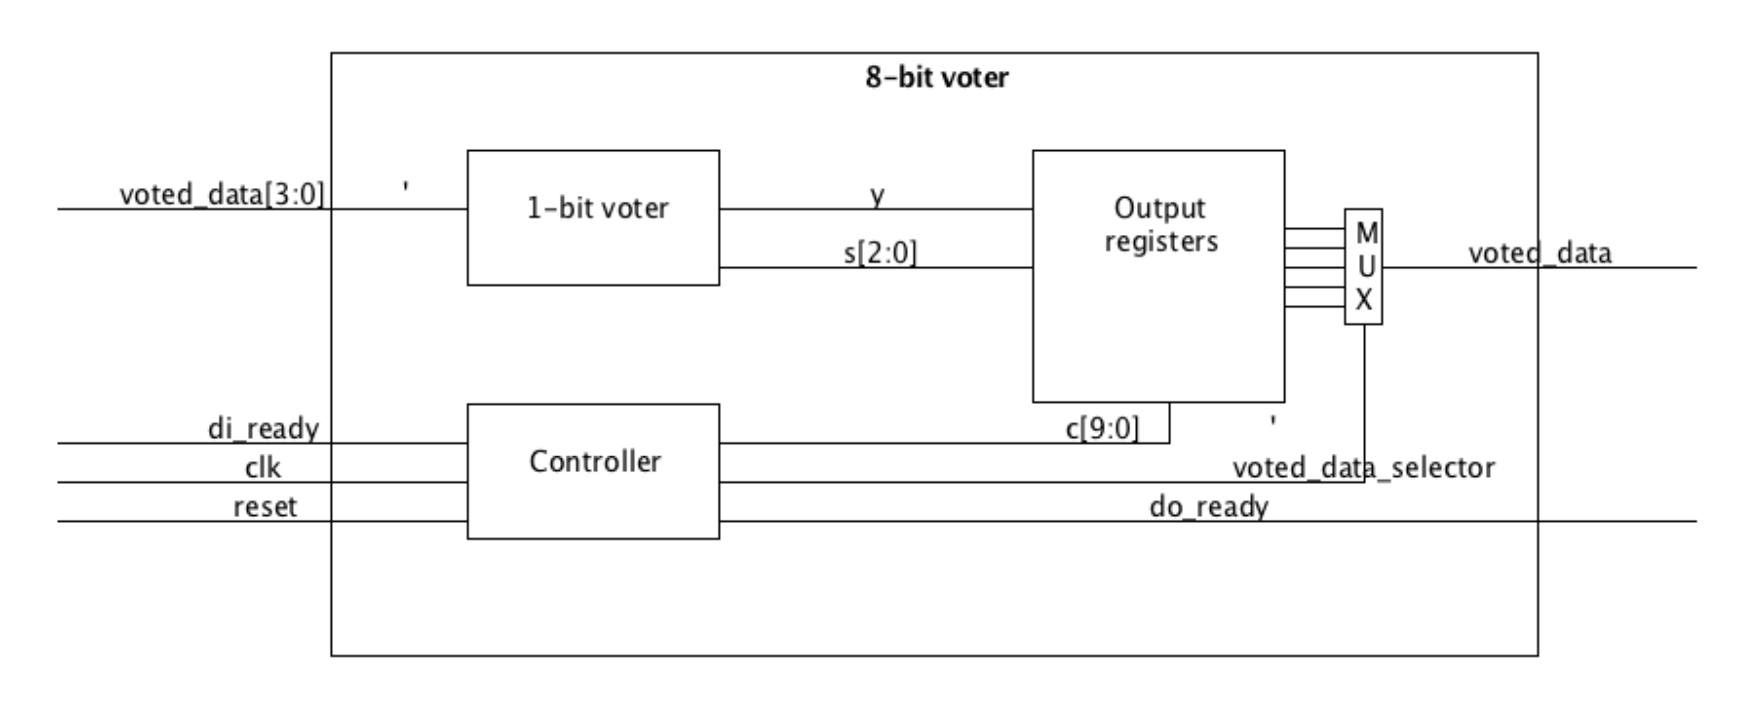
\includegraphics[width=0.5\textwidth]{Figures/Solution/ArchitectureOption1}
    \caption{Optional architecture for the 8-bit Voter: Using 1-bit voter and registers}
    \label{fig:ArchitectureOption1}
\end{figure}
Figure \ref{fig:ArchitectureOption1} shows a component based implementation that includes the 1-bit voter, a controller module, a register module and a multiplexer. Data are received serially, voted serially by the 1-Bit Voter, and the resulting data are stored in registers. After a specified number of cycles, data are to be sent out serially, together with the \textit{do\_ready} signal.
\begin{figure}[h!]
    \centering
    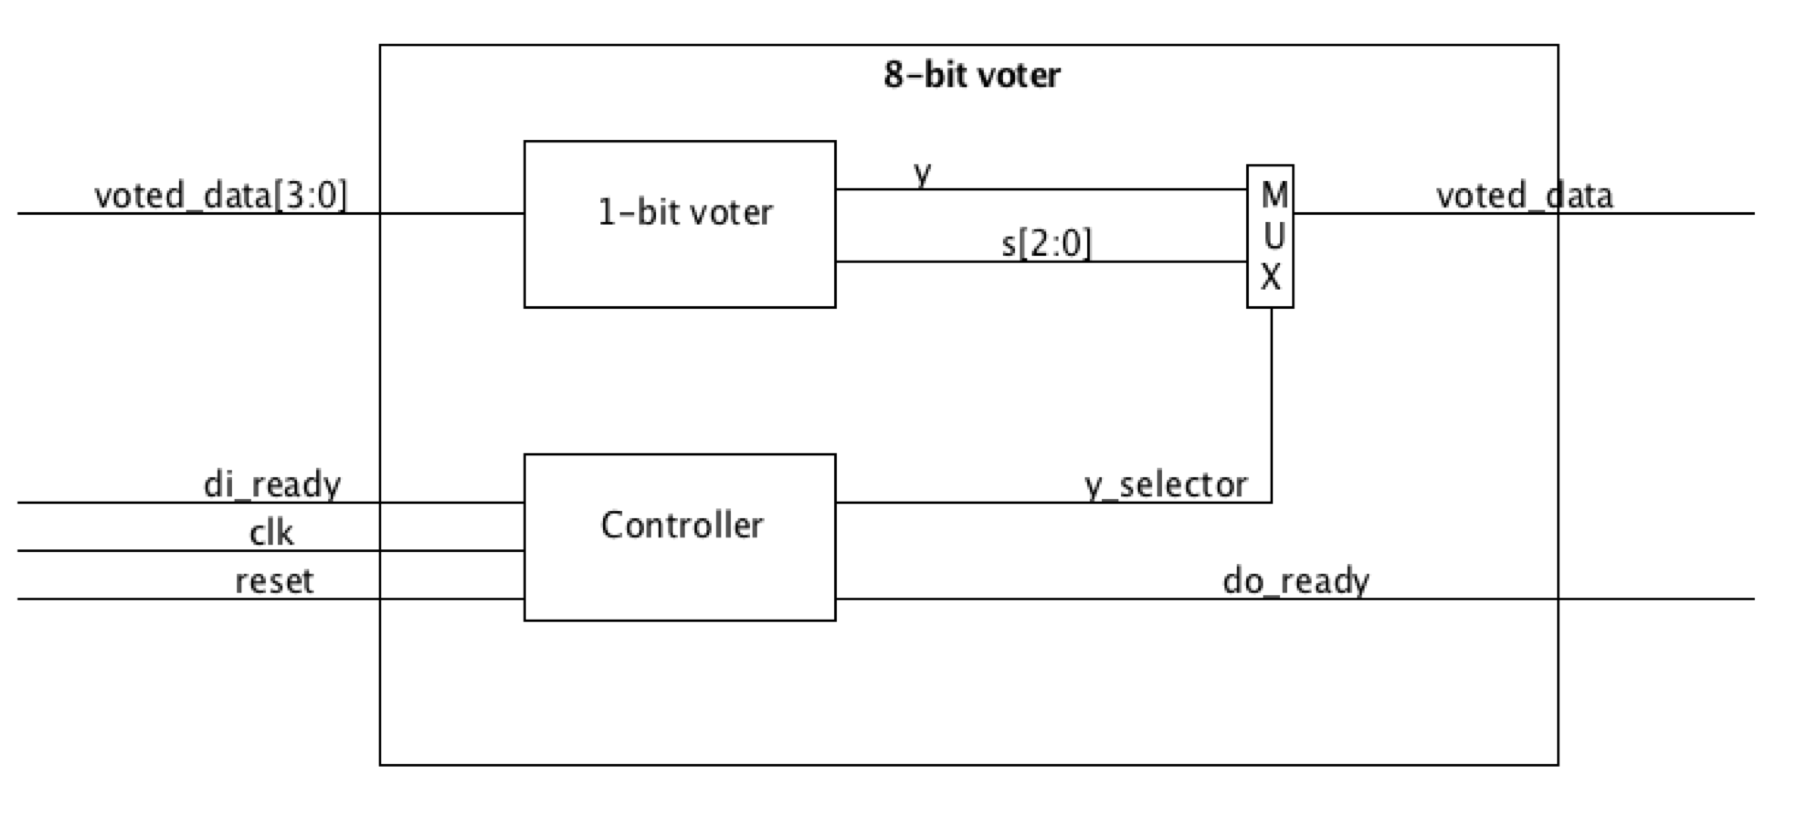
\includegraphics[width=0.5\textwidth]{Figures/Solution/ArchitectureOption2}
    \caption{Optional architecture for the 8-bit Voter: Not using registers}
    \label{fig:ArchitectureOption2}
\end{figure}
Figure \ref{fig:ArchitectureOption2} shows an option where no registers are implemented. 
The idea is to have as small 8-Bit Voter as possible. 
Data that are read and voted serially must be passed on immediatly.

\begin{figure}[h!]
    \centering
    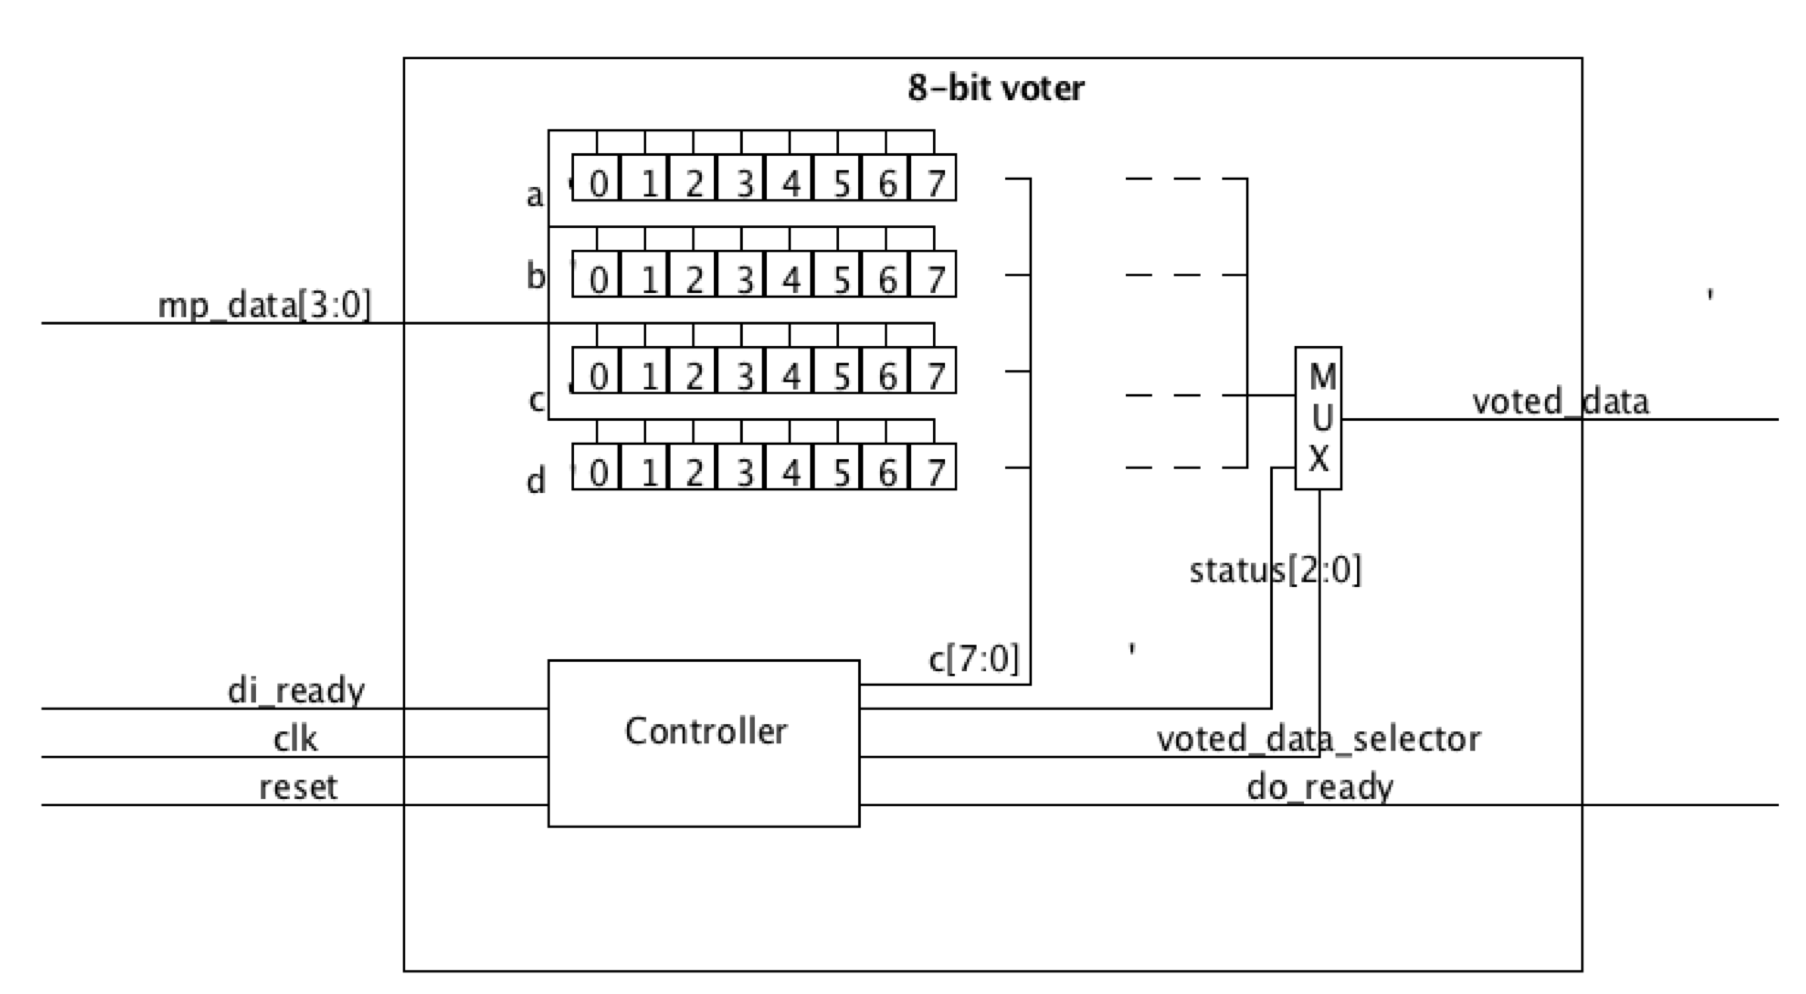
\includegraphics[width=0.5\textwidth]{Figures/Solution/ArchitectureOption3}
    \caption{Optional architecture for the 8-bit Voter: Not using 1-bit voter}
    \label{fig:ArchitectureOption3}
\end{figure}
Figure \ref{fig:ArchitectureOption3} shows an option where the 1-Bit Voter is not used. In this scenario, 4 sets of 8-Bit words are stored and voted.
Though the voting can be done serially for each arrived sets of bits, the idea is that it can also perform instant voting on the entire 8 bit words.
Note that output status data must be handled differently in lack of the designed 1-Bit Voter.
The Controller has this responsibility in this case.

\subsubsection{Choice of Archtecture}
While the second option uses less space than the first one, and it is possible to pass on data immediatly as soon as it arrives, the Term Assignment specifies that the ECC module is to be imeplemented using Hamming Codes.
The ECC calculation cannot be done before all data have arrived, voting is done and the status bits are updated.
But with this implementation, the data is sent immediatly, but not stored.
The ECC module will have to implement registers, but this contradicts the idea behind this option of not using registers.
The second option is thus not compatible with expanding the system with an ECC module.
\break
The third option uses another solution than a 1-Bit voter, but the group conciders the 1-Bit Voter to be sufficient.
Implementing another voter is concidered a waste of time since there is already a solution available, that the group conciders to be good enough.
All data arrives serially, and are sent out serially from the Liasion, and serial voting between receiving and sending is sufficient.
If all received data were to be voted instantly by voting the entire word, it would create constriction on receiving data and sending out data.
Only status data or ECC data from the previous vote can be sent out while an 8-bit voting is performed.
Though maximum throughput is possible, the design is more difficult to implement.
This solution is likely to have greater complexity than the first option, and the use of four sets of registers make the 8-Bit Voter conciderably larger than the first option.
Given these premises, the group has chosen to implement the first option, since the other options are concidered weaker.
The full architecture, which includes the ECC module, can be seen in figure \ref{fig:ArchitectureFinal}.
Note that this is named Liasion, since it is used as topmodule for the Liasion system.

\begin{figure}[h!]
    \centering
    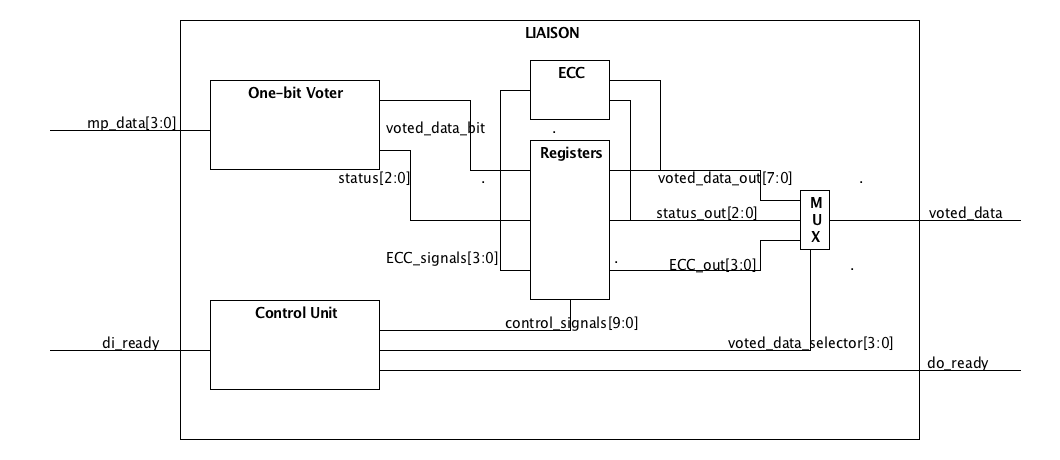
\includegraphics[width=0.5\textwidth]{Figures/Solution/ArchitectureFinal}
    \caption{Chosen architecture for the 8-bit Voter}
    \label{fig:ArchitectureFinal}
\end{figure}

\subsubsection{The Register Module}
\begin{figure}[h!]
    \centering
    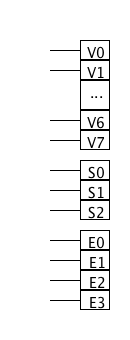
\includegraphics[width=0.10\textwidth]{Figures/Solution/Registers}
    \caption{Implemented registers}
    \label{fig:Registers}
\end{figure}
Figure \ref{fig:Registers} shows the contents of the register modules.
There are 8 registers for storing voted data and 3 for storing status data from the 1-Bit Voter.
The group has chosen to implemen 4 bits of ECC data in this project.
The register module is controlled by a 10-bit control\_signal, that is used when storing data.
The control\_signal, which is set by the control\_unit, has 1 bit for every 8 voted data register, since voted data arrive serially and must be stored one by one.
The 9th bit is used for storing data in the status registers, since all 3 status bits arrive simultaniously.
The 10th bit is used for storing data in the ECC registers, since ECC data are calculated and thus stored thenext  cycle after being done with all voted data and status data.
If none of these control bits are active, no new data will be stored.

\subsubsection{The Controller Module}
The Controller Module is responsible for controlling the registers when storing data, and setting the multiplexer so that correct data is sent out per cycle.
The module is implemented as two state machines.
\begin{figure}[h!]
    \centering
    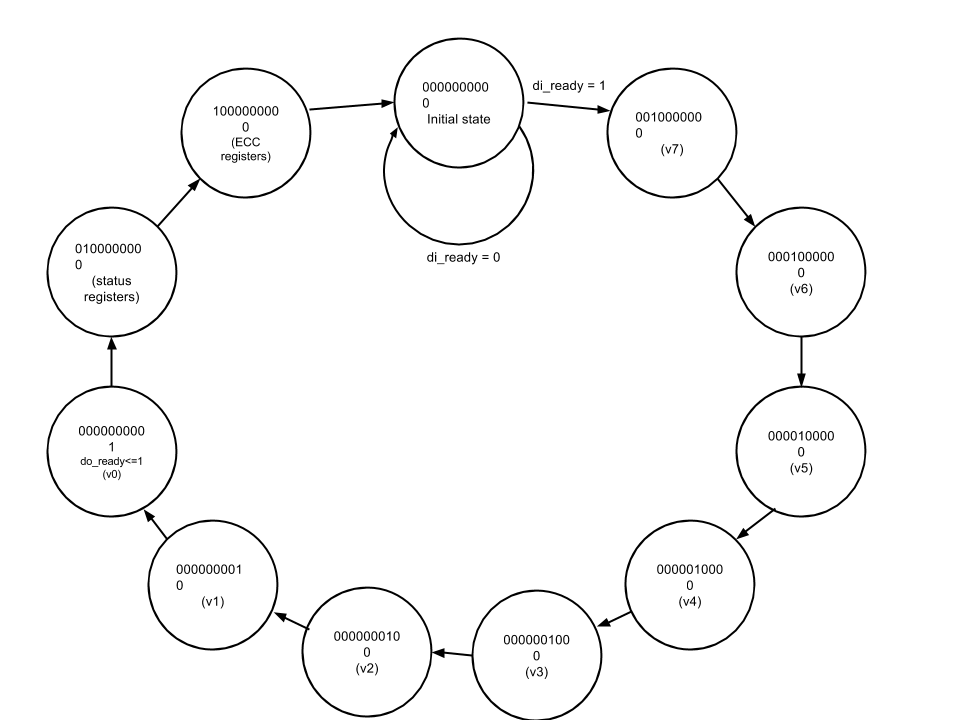
\includegraphics[width=0.50\textwidth]{Figures/Solution/ControllerStateMachine1}
    \caption{Controller state machine 1}
    \label{fig:ControllerStateMachine1}
\end{figure}
Figure \ref{fig:ControllerStateMachine1} shows the first state machine.
It is activated by the \textit{di\_ready} signal, and sets the 10-bit \textit{control\_signal} that is connected to the register module.
After a specified number of cycles, in this case 7 after \textit{di\_ready}, the \textit{do\_ready} pulses for one cycle.
It can also be seen in the figure which registers are affected by the different states.
Though it is not seen in the figure, if the \textit{reset} signal is activated, the initial state is set.
\begin{figure}[h!]
    \centering
    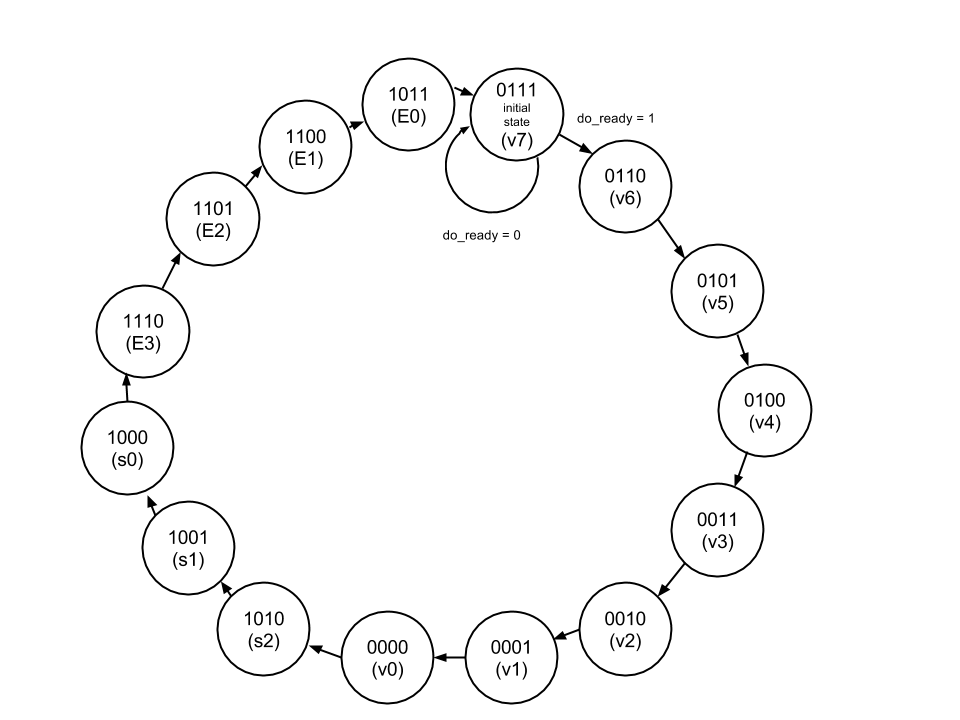
\includegraphics[width=0.50\textwidth]{Figures/Solution/ControllerStateMachine2}
    \caption{Controller state machine 2}
    \label{fig:ControllerStateMachine2}
\end{figure}
Figure \ref{fig:ControllerStateMachine2} shows the second state machine.
It is activated by the \textit{do\_ready} signal, and sets the 4-bit control\_signal{4-bit voted\_data\_selector} that is connected to the multiplexer, so that data from the registers are sent out in the correct order.
This figure shows as well the connection between the output and the registers, and though it is not seen, an active \textit{reset} will return the machine to the initial state.
There are 7 cycles before activating the second state machine, and 15 cycles for the second state machine for setting the output data.
In total this makes up 22 cycles before going idle, should there be no more \textit{di\_ready} signals.
If the next \textit{di\_ready} signal arrives too early, it will have to be ignored, since the shortest possible intervals for the system are 15 cycles.

\subsection{Sub-Problem 4: Error Correction Circuit}
When transmitting data there is always a risk of the data being received with one or more bits flipped.
This effect pose a way greater threat when the datatransmission is a wireless transmission from a small satelite in space.
To battle this effect the Liaison system feature an error correcting circuit that add 4 bits to each transmission.
This mean that every set of 8 bits from the microcontrollers will be accompanied by not only the 3 status bits, but also 4 bits that provide confidence in the other 11.

\begin{figure}[h!]
\begin{lstlisting}
data_out(0) <= data_in(0) xor data_in(1) xor data_in(3) xor data_in(4) xor data_in(6) xor data_in(8) xor data_in(10);
data_out(1) <= data_in(0) xor data_in(2) xor data_in(3) xor data_in(5) xor data_in(6) xor data_in(9) xor data_in(10);
data_out(2) <= data_in(1) xor data_in(2) xor data_in(3) xor data_in(7) xor data_in(8) xor data_in(9) xor data_in(10);
data_out(3) <= data_in(4) xor data_in(5) xor data_in(6) xor data_in(7) xor data_in(8) xor data_in(9) xor data_in(10);
\end{lstlisting}
\caption{The hamming code example from the staff in TFE4140 \protect\cite{hamming-codes}.}
\label{fig:HammingCodeLogic}
\end{figure}
Based on the logic from the example ECC module\protect\cite{hamming-codes} constructing a module for the liaison system was straight forward.
The module is a simple combinatorial module that continously read the states of the voted data and status registers.
Whenever one of these registers are updated, the ECC module will also update it's value.
It is the then up the the control unit to write the values from the ECC at the right point of time.

\subsection{Sub-Problem 5: Analysis of error probabilities}
A microcontroller is expected to fail on an avarage of 6 years.
Sub-Problem 5 of the Term Assignment specified that 3 mathematical expressions on failure after a time \textit{t}, as well as Mean Time To Failure (MTTF) for the system are to be calculated:
\begin{itemize}
    \item The probability for error in maximum one controller (that is zero or one) after \textit{t} time. This will be expressed as P(Max(1)). 
    \item The probability for error in maximum two controllers after \textit{t} time. This will be expressed as P(Max(2)).
    \item The probability for error at least three controllers after \textit{t} time. This will be expressed as P(Least(3)).
    \item The MTTF for the whole system.
\end{itemize}

The propability that a machine does not fail after a time \textit{t}, given the expected life time \textit{T}, is expressed as $P = P(t) = e^{-t/T}$.
Since the expected life time for a microcontroller is T = 6, the probability is expressed as $P = P(t) = e^{-t/6}$. 
The different probabilites that are calculated are:
\begin{itemize}
    \item $P(Max(1)) = e^{-t/2}+3(e^{-t/2}-e^{-2t/3})$
    \item $P(Max(2)) = 3e^{-2t/3}-8e^{-t/2}+6e^{-t/3}$
    \item $P(Least(3)) = 1-3e^{-2t/3}+8e^{-t/2}-6e^{-t/3}$
    \item MTTF = 6.5 years.
\end{itemize}

These calculations and how they are done are explained in full details in Appendix C.

\section{ Testing and verification }
\subsection{ Testing and verification }
To ensure correct funtionallity of each of the modules, and the liaison system as a whole, they are all covered by testbenches.
These testbenches simulate the behaviour of the modules and expose all potential errors in the system.
All such errors can then be fixed, and the result is a fully functioning system.
All the tests were also ran post synthesis through Synplify Pro.
This section will present what were tested in each component, and the final test results.

\subsection{ Tests and verification of 1-Bit Voter}
Originally, each member of the group created a test bench of their own for their 1-Bit Voters, as part of assignment 3.
The group later received a test bench from the course staff for the evaluation of assignment 3, and this has replaced the old test benches.
The reason behind this choice is that the group conciders the scenario in the test bench to be realistic for all situations.
It is not likely that there will arise other situations when it comes to inputs and behaviour of the module as is tested in this test bench.
Therefore the group conciders this test bench to do full coverage of the 1-Bit Voter.
The test bench compares outputs with expected results, and throws an error whenever there is a difference between test outputs and expected outputs.
Different combinations of inputs are tested, and one by one microcontroller are set to fail.
The failed microcontrollers are tested for error tagging by testing whether their data has any affection on the output \textit{voted\_data}.
\textit{Reset} is always activated to reset and test for other input combinations.
The entire test passes with the current 1-Bit Voter. 
\todo{ Explain test results. Include screenshot (Uh... the provided test bench is not of that kind).}

\subsection{ Controller Module}
The Controller Module is tested for these different situations:
\begin{itemize}
    \item \textbf{Long intervals between \textit{di\_ready}}. 
        The controller should set it's outputs so that only the one stream of input data associated with the received \textit{di\_ready} signal should be stored and sent out of the Liasion module.
        This is seen in the test as changes in the outputs of the module.
        These changes should be traversed only once per \textit{di\_ready}, and is expected to last for 22 \todo{ Count in test} cycles.
    \item \textbf{Too short intervals between \textit{di\_ready}}.
        The controller should ignore \textit{di\_ready} signals that arrive too early, since the system is not finished receiving and/or processing the current data.
    \item \textbf{Maximum throughput}.
        The controller should enable maximum througput when \textit{di\_ready} signals are received every 15 cycles.
        This can be seen as there are changes on the output \textit{voted\_data\_selector} at every clock cycle.
    \item \textbf{Reset}.
        Whenever the \textit{reset} signal pulses, the controller should synchronously halt any activity, and reset both state machines and outputs to initial value.
        Any waiting \textit{do\_ready} signal should not be sent out.
        Reset is tested for both before activating second state machine, and after. 
\end{itemize}
These are the different situations that might occur for the controller module, therefore this test is concidered to give full coverage for the controller module.

\begin{figure}[h!]
  \centering
      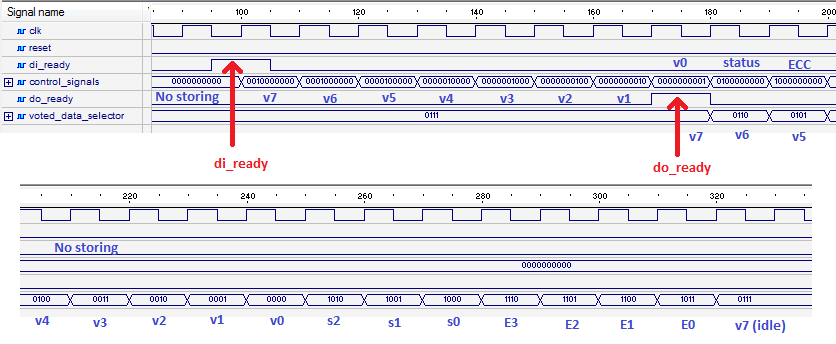
\includegraphics[width=0.5\textwidth]{Figures/Tests/ControllerRegular}
  \caption{Screenshot from Controller test: A full regular message transmission cycle.}
  \label{fig:ControllerRegular}
\end{figure}
Figure \ref{fig:ControllerRegular} shows a regular data transmission cycle in the controller after the \textit{di\_ready} signal pulses.
The output for register storing are set accordingly for every cycle, \textit{do\_ready} pulses after 7 cycles, and the output to the multiplexer are set afterwards for each cycle. 
he outputs in the figure are tagged to show what data are stored, and what data are to be sent out based on the control signals.
Notice that when idle, the multiplexer is set to constantly reading v7.

\begin{figure}[h!]
  \centering
      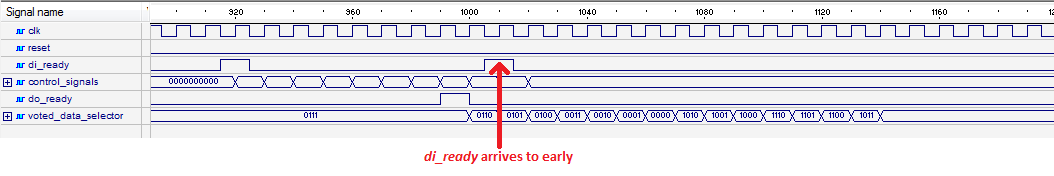
\includegraphics[width=0.5\textwidth]{Figures/Tests/ControllerTooEarlyDiReady}
  \caption{Screenshot from Controller test: Too early \textit{di\_ready}.}
  \label{fig:ControllerTooEarlyDiReady}
\end{figure}
Figure \ref{fig:ControllerTooEarlyDiReady} shows an example where the signal \textit{di\_ready} arrives too soon after the previous one.
What happens is that it is simply ignored, and no additional data are stored and sent out in addition to the data that is already being processed.

\begin{figure}[h!]
  \centering
      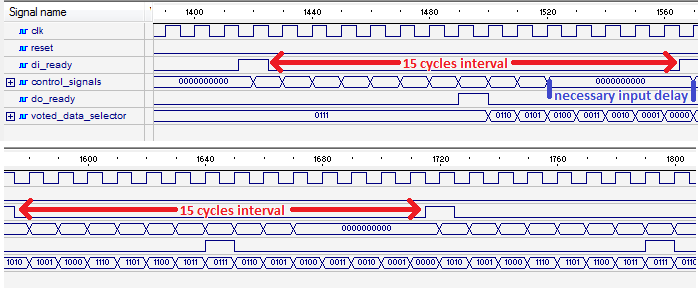
\includegraphics[width=0.5\textwidth]{Figures/Tests/ControllerThroughput}
  \caption{Screenshot from Controller test: Maximum throughput.}
  \label{fig:ControllerThroughput}
\end{figure}
Figure \ref{fig:ControllerThroughput} shows that when the interval between the \textit{di\_ready} signals are 15 cycles, the output to the multiplexer changes every cycle, which is consistent with sending out data bits from the Liasison system every cycle.
Also notice that there are some delays on the control signal for input storing.

\begin{figure}[h!]
  \centering
      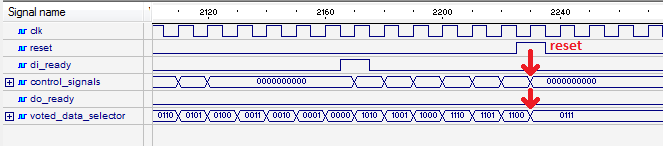
\includegraphics[width=0.5\textwidth]{Figures/Tests/ControllerReset}
  \caption{Screenshot from Controller test: Reset is active.}
  \label{fig:ControllerReset}
\end{figure}
Figure \ref{fig:ControllerReset} shows that when reset is active, the controller is reset and the outputs are set to their idle values.

\subsection{ ECC }
\todo{ Explain choice of test bench. Explain why only partial coverage is enough. }
\break
\break
\todo{ Explain test results. Include screenshot. }

\subsection{ Liaison }
The test bench for the Liaison system is a test of the top level.
The behaviour of the Liaison relies heavily on the 1-Bit Voter and the Controller Module.
These two components are already tested in full coverage, therefore most of the Liasion is indirectly tested.
The test bench gives thus only partial cover, only to do a small control to ensure that the components and the toplevel cooperate as expected.

\begin{figure}[h!]
    \centering
    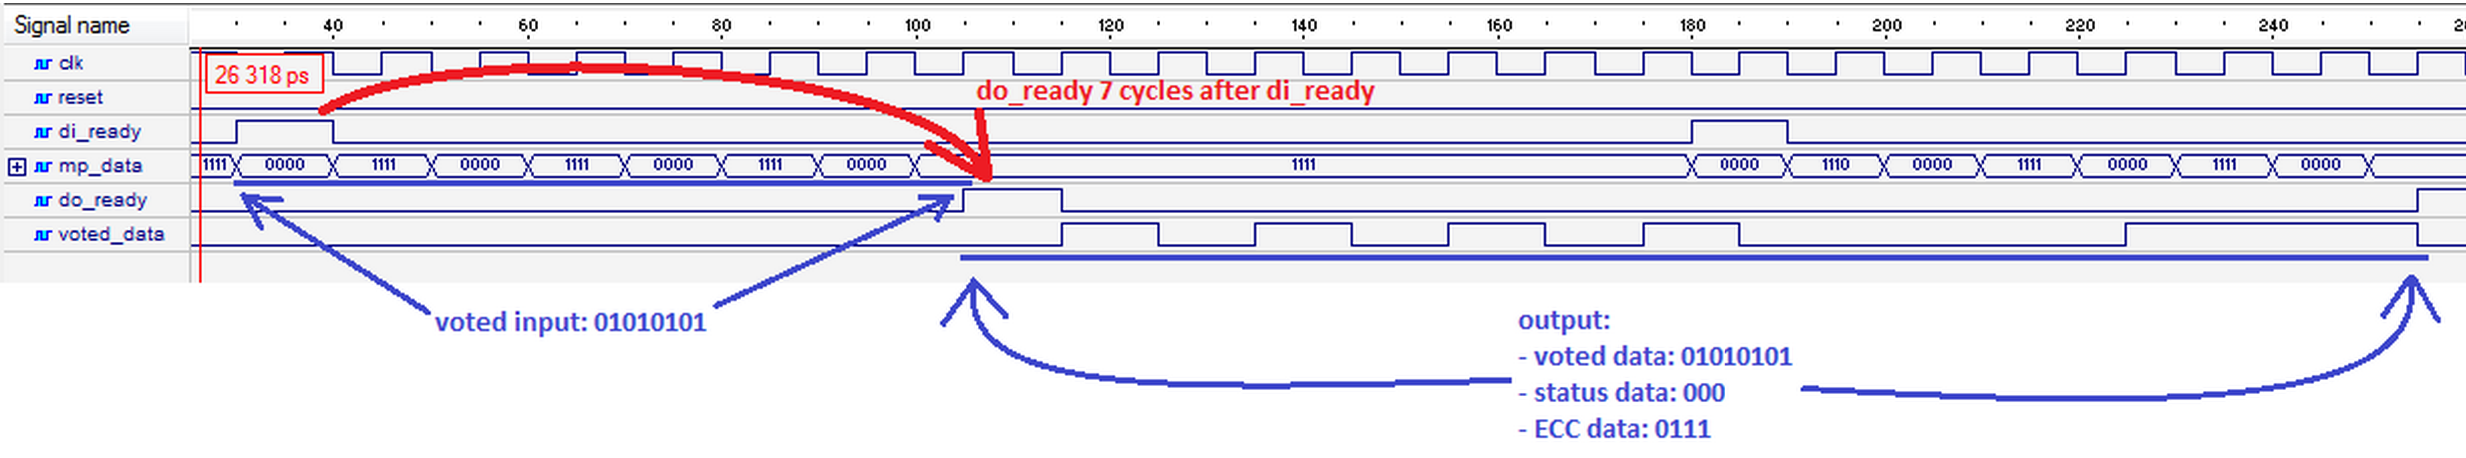
\includegraphics[width=0.5\textwidth]{Figures/Tests/LiaisonTest}
    \caption{Screenshot from Liaison Test}
    \label{fig:LiaisonTests}
\end{figure}

Figure \ref{fig:LiaisonTests} shows a screenshot of the test output.
The red arrow marks the interval between the \textit{di\_ready} and the \textit{do\_ready}, illustrating that the first activates the second.
The inputs are also markes, and are sent out as the 8 first bits of the output.
The output also includes status bits and ECC bits.
The output of this tests show that the components cooperate as expected.
This depends on that each component works as expected, but that is already tested in the other test benches.

\section{Synthesis Results}
Both members of the team implemented one 1-Bit Voter each and synthesized them, according to course assignments 3 and 4.
Torbjørn Langland's 1-Bit Voter had a resulting estimated frequency of 230.2 MHz, and 73 LUTs, which is concidered to be mediocre.
Rune Holmgren's Voter had a resulted estimated frequency of 423 MHz and 33 LUTs, which was clearly much better.
Rune's Voter was chosen for the implementation of the Liaison system.
It has also been futher optimalized in the latter stages of the project.
The final resulting number of LUTs implemented in the system is:
\begin{itemize}
    \item 1-Bit Voter: 27
    \item Controller: 18
    \item ECC: 9
    \item Registers: 0
    \item Toplevel: 8
    \item \textbf{Total: 62}
\end{itemize}
Total number of flip-flops in the system is: 52.
\break
Estimated frequency of the system is: 213.7 MHz
\break
The resulting Schematics for both RTL view and Technology view are detailed in Appendix B.

\section{Feedback and other Information}
\todo{ The teachers wanted feedback. They also want to know the time spent on the work. This is where it should be added}.
\subsection{Feedback}
\todo{ The cake is a lie!}

\subsection{Time spent by the group}
Rune Holmgren has recorded a total number of 95 hours spent on this project.
\break
Torbjørn Langland was unfortunate and broke his computer by spilling coffee on it.
His record data which contained the information about time spent on the project was stored on it, therefore the total number of hours spent is now unknown.
\todo{ Mention agreement with the teacher that estimation is accepted?}
He estimates that he has spent roughly about 70 hours on this project before this incident.
With the logged activity after the incident Torbjørn estimates to have spent a total number of XX hours on this project.
This includes writing this report.
\todo{ Fill in spent hours at last, since report also counts as work}
\todo{insert details of how much time spent on the project, including on this report.}

\section{Conclusion}
\todo{ Compulsory. Have a good wrap up, somehow. }

\section{Acknowledgements (optional)}
The group would like to extend their sincere thanks to the following individuals:
\begin{itemize}
    \item Group 2 with Solveig Fure and Erick Castillo, for review and feedback of the project.
    \item Student assistent Kyrre Erlend Gonsholt for helping out in situations where we were stuck.
    \item Indiana Jones. \todo{ ! }
\end{itemize}


\section{ Other problems/needs to be solved:}
\subsection{ Appendixes}
\todo{ Appendix A: Project code }
\break

\bibliography{bibliography}
\bibliographystyle{plain}
\nocite{*}

\clearpage
\begin{titlepage}
    \newcommand{\HRule}{\rule{\linewidth}{0.5mm}} % Defines a new command for the horizontal lines, change thickness here
    \center % Center everything on the page
    \vspace*{3cm}
    \HRule \\[0.4cm]
    { \huge \bfseries Appendices}\\[0.4cm] % Title of your document
    \HRule \\[1.5cm]
\end{titlepage}
\clearpage

% Appendix A
\begin{titlepage}
    \newcommand{\HRule}{\rule{\linewidth}{0.5mm}} % Defines a new command for the horizontal lines, change thickness here
    \center % Center everything on the page
    \vspace*{3cm}
    \HRule \\[0.4cm]
    { \huge \bfseries Appendix A}\\[0.4cm] % Title of your document
    \HRule \\[1.5cm]
    All code in this appendix is also availabe from : \break \href{https://github.com/Raane/Term-Assigment-TFE4140-mod-anal-dig-sys}{https://github.com/Raane/Term-Assigment-TFE4140-mod-anal-dig-sys}
%one bit voter
\begin{figure}[h!]
    \lstinputlisting[firstline=0, lastline=65]{../Project/liaison/src/onebitvoter.vhd}
\caption{onebitvoter.vhd part 1}
\end{figure}
\begin{figure}[h!]
    \lstinputlisting[firstline=66, lastline=130]{../Project/liaison/src/onebitvoter.vhd}
\caption{onebitvoter.vhd part 2}
\end{figure}
\begin{figure}[h!]
    \lstinputlisting[firstline=131, lastline=191]{../Project/liaison/src/onebitvoter.vhd}
\caption{onebitvoter.vhd part 3}
\end{figure}

%liaison
\begin{figure}[h!]
    \lstinputlisting[firstline=0, lastline=65]{../Project/liaison/src/liaison.vhd}
\caption{liaison.vhd part 1}
\end{figure}
\begin{figure}[h!]
    \lstinputlisting[firstline=66, lastline=117]{../Project/liaison/src/liaison.vhd}
\caption{liaison.vhd part 2}
\end{figure}

%Registers
\begin{figure}[h!]
    \lstinputlisting[firstline=0, lastline=65]{../Project/liaison/src/registers.vhd}
\caption{registers.vhd part 1}
\end{figure}
\begin{figure}[h!]
    \lstinputlisting[firstline=66, lastline=76]{../Project/liaison/src/registers.vhd}
\caption{registers.vhd part 2}
\end{figure}

%Controller
\begin{figure}[h!]
    \lstinputlisting[firstline=0, lastline=65]{../Project/liaison/src/controller.vhd}
\caption{controller.vhd part 1}
\end{figure}
\begin{figure}[h!]
    \lstinputlisting[firstline=66, lastline=130]{../Project/liaison/src/controller.vhd}
\caption{controller.vhd part 2}
\end{figure}
\begin{figure}[h!]
    \lstinputlisting[firstline=131, lastline=140]{../Project/liaison/src/controller.vhd}
\caption{controller.vhd part 3}
\end{figure}

%ECC
\begin{figure}[h!]
    \lstinputlisting{../Project/liaison/src/ECC.vhd}
\caption{ECC.vhd}
\end{figure}

\end{titlepage}
\clearpage

% Appendix B
\begin{titlepage}
    \newcommand{\HRule}{\rule{\linewidth}{0.5mm}} % Defines a new command for the horizontal lines, change thickness here
    \center % Center everything on the page
    \vspace*{3cm}
    \HRule \\[0.4cm]
    { \huge \bfseries Appendix B}\\[0.4cm] % Title of your document
    \HRule \\[1.5cm]
\end{titlepage}
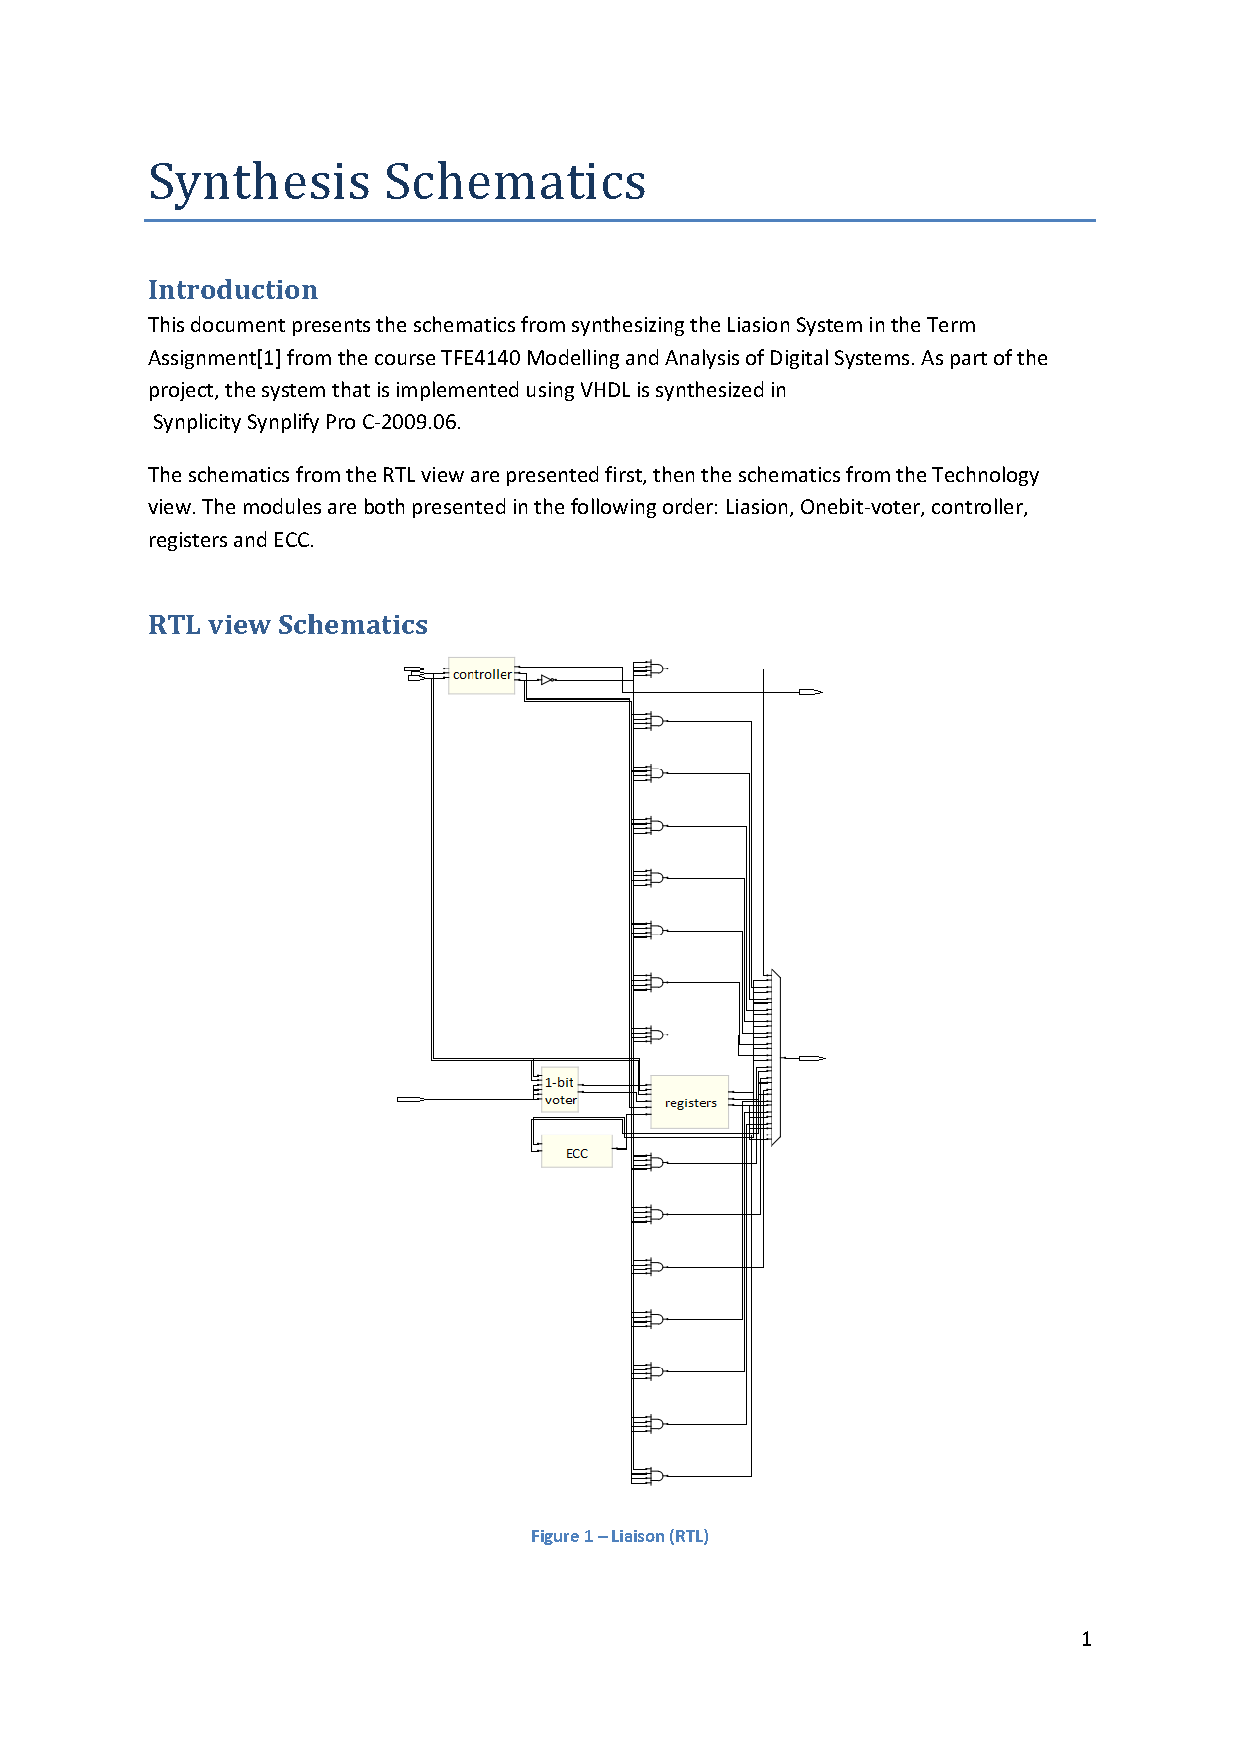
\includepdf[pages={1,2,3,4,5,6,7,8}]{Appendixes/AppendixB.pdf}
\clearpage

% Appendix C
\begin{titlepage}
    \newcommand{\HRule}{\rule{\linewidth}{0.5mm}} % Defines a new command for the horizontal lines, change thickness here
    \center % Center everything on the page
    \vspace*{3cm}
    \HRule \\[0.4cm]
    { \huge \bfseries Appendix C}\\[0.4cm] % Title of your document
    \HRule \\[1.5cm]
\end{titlepage}
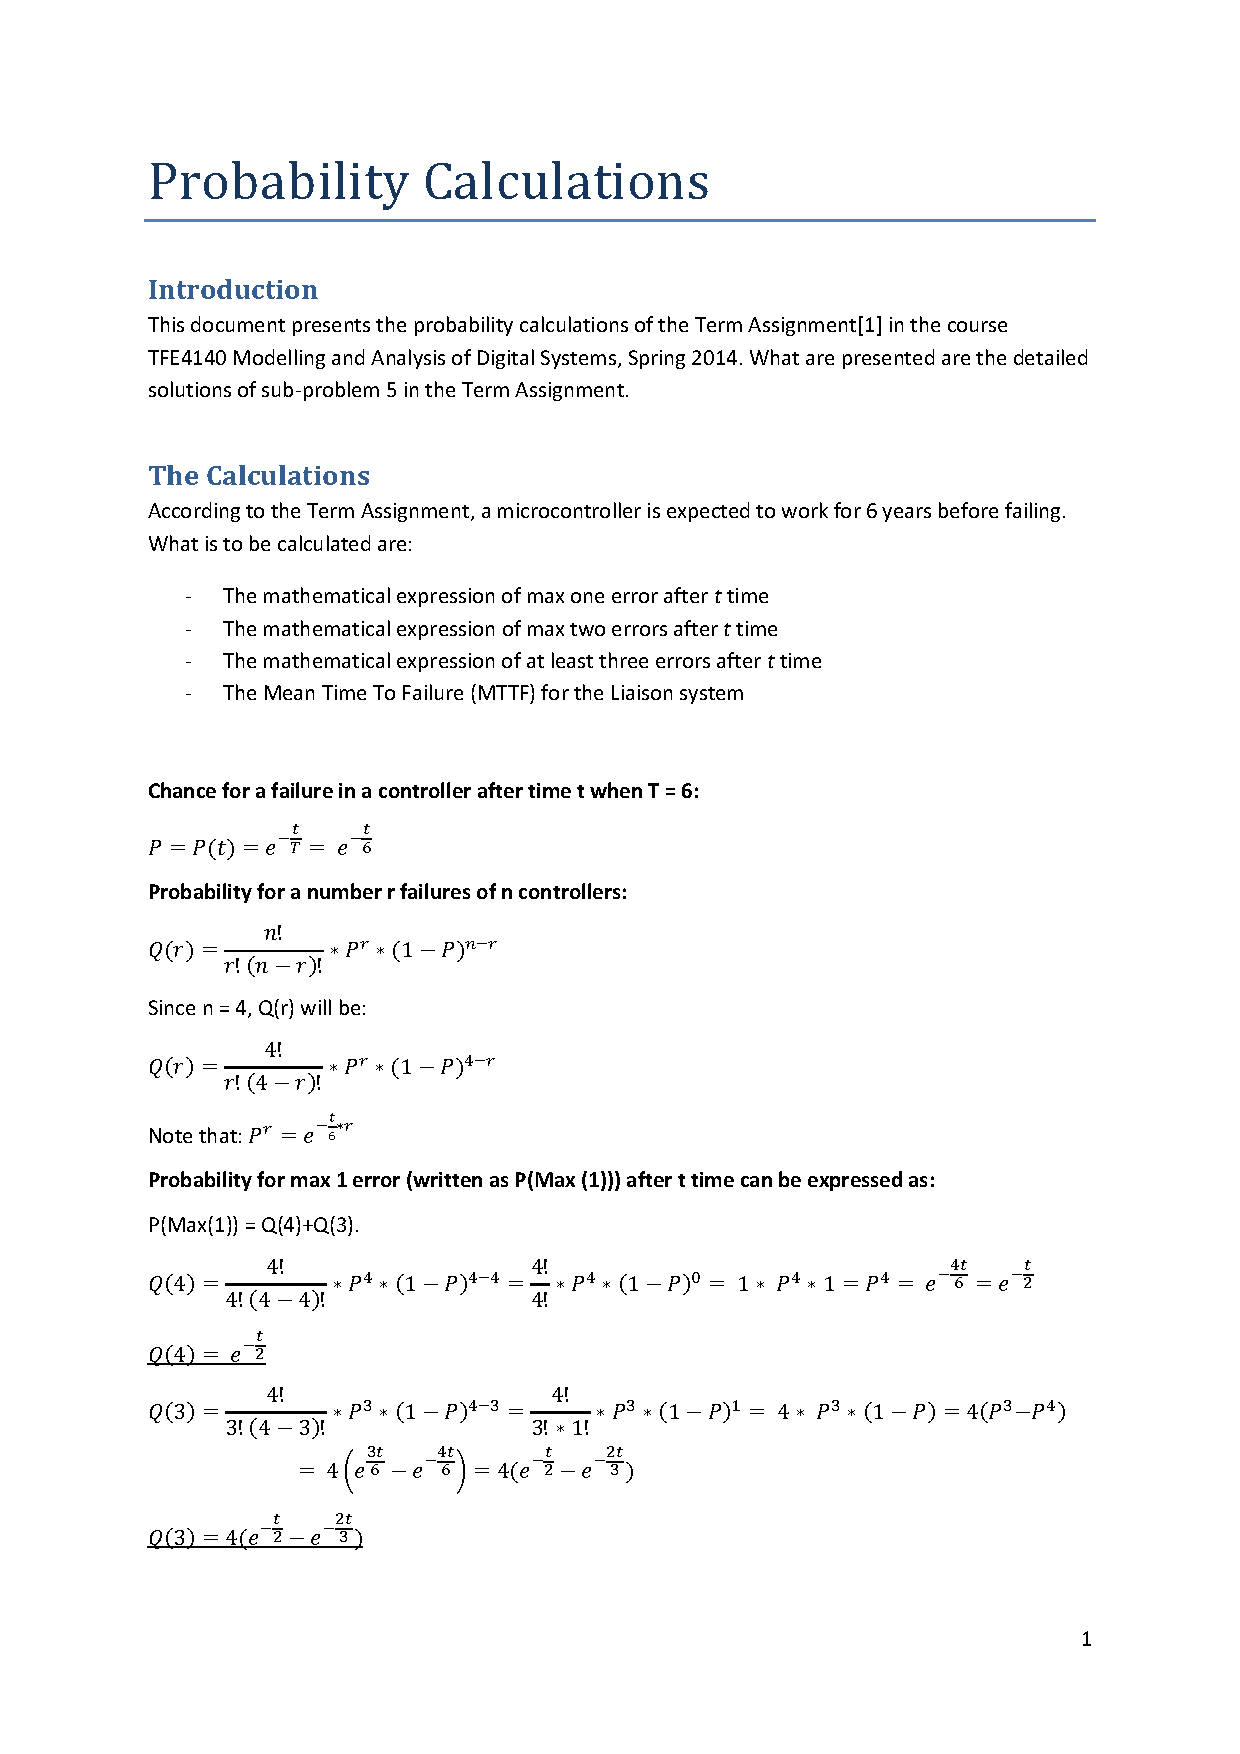
\includepdf[pages={1,2,3,4}]{Appendixes/AppendixC.pdf}

\end{document}
